%DO NOT MESS AROUND WITH THE CODE ON THIS PAGE UNLESS YOU %REALLY KNOW WHAT YOU ARE DOIN

\chapter{Implementation and Methodology} \label{Implementation and Methodology}

\section{Tools Used } \label{Tools Used }
\noindent The following Tools have been used for implementation.
\subsection{Microsoft Kinect v2 sensor} \label{Microsoft Kinect v2 sensor} 
\noindent Specifications of the Kinect are discussed in Chapter 3.
\subsection{Visual Studio 2015 Community Edition }\label{Visual Studio 2015 Community Edition }  
\noindent Microsoft Visual Studio is an integrated development environment (IDE) from Microsoft. It is used to develop computer programs for Microsoft Windows, as well as web sites, web apps, web services and mobile apps. Visual Studio uses Microsoft software development platforms such as Windows API, Windows Forms, Windows Presentation Foundation, Windows Store and Microsoft Silverlight. It can produce both native code and managed code.\\
\noindent Visual Studio supports different programming languages and allows the code editor and debugger to support (to varying degrees) nearly any programming language, provided a language-specific service exists. Built-in languages include C, C++and C++/CLI (via VisualC++), VB.NET (via VisualBasic.NET), C\# (via Visual C\#), and F\# (as of Visual Studio 2010). Support for other languages such as Python, Ruby, Node.js, and M among others is available via language services installed separately.
\noindent Microsoft provides the Kinect SDK and Kinect specific libraries to be used on Visual Studio. This is the reason we have chosen Visual Studio as our development platform as it makes interfacing the Kinect easy.   
\subsection{Notepad++ }\label{Notepad++ } 
\noindent Notepad++ is a text editor and source code editor for use with Microsoft Windows. It supports tabbed editing, which allows working with multiple open files in a single window. Notepad++ is distributed as free software. It supports syntax highlighting and code folding for over 50 programming, scripting, and markup languages.\\
The skeletal data obtained from the SDK is stored in CSV format in a Notepad++.

\subsection{MATLAB R2015a }\label{MATLAB R2015a }
\noindent MATLAB is a multi-paradigm numerical computing environment and fourth-generation programming language. A proprietary programming language developed by MathWorks, MATLAB allows matrix manipulations, plotting of functions and data, implementation of algorithms, creation of user interfaces, and interfacing with programs written in other languages, including C, C++, C\#, Java, Fortran and Python.\\
MATLAB provides special toolboxes for applications such as Signal Processing and Communications, Control System Design and Analysis, Pattern Recognition, Classification Learner and other statistical modelling \\
The CSV format file is processed in MATLAB for gait feature extraction and classification. 

\section{Gait Features} \label{Gait Features } 
\noindent The Kinect SDK offers the detection and tracking of 25 different skeletal joints. The features that can be generated from these joints can broadly be classified as static and kinematic features.
The static features are the ones which do not change in time as a person is walking, for e.g. Height.
We define a set of 7 static features used in our study


\begin{table}
\centering
\begin{tabular}{| l | |p{5cm}|}
 \hline
SR No. & Static Features  \\ \hline
1 & Height \\ \hline
2 & Length of Full Arms \\ \hline
3 & Length of Fore Arms \\\hline
4 & Length of Upper Arms \\ \hline
5 & Length of Full Legs \\ \hline
6 & Length of Thighs \\\hline
7 & Length of Lower Legs \\ \hline

\end{tabular}
\caption{The set of static features}
\end{table}



\noindent Kinematic features basically involve distance and angle between joints while a person is walking. These value of these features constantly change during the walking and are shown to be periodic in nature.
We define a set of 8 kinematic features involving distance between joints 

\begin{table}
\centering
\begin{tabular}{| l | |p{6cm}|}
 \hline
SR No. & Features  \\ \hline
1 & Distance between ankles \\ \hline
2 & Distance between knees \\ \hline
3 & Distance between elbows \\\hline
4 & Distance between hands \\ \hline
5 & variance of head (along x) \\ \hline
6 & variance of head (along y) \\\hline
7 & variance of left knee (along y) \\ \hline
8 & variance of right knee (along y) \\ \hline
\end{tabular}
\caption{ kinematic features involving distance between joints}
\end{table}

\noindent When we talk about the features such as variance of head and knees along X and Y. We are trying to map the vertical and lateral oscillations of these skeleton joints.

\noindent Features involving angles are extracted during the walk but are not used in this study and will be discussed later. Here we would like to divide our implementations into two parts

\noindent$\bullet$ Part I  : This will deal with the experimental setup, design of the application using the Kinect SDK, logic behind measurements of static and kinematic features and their extraction.\\
The tasks discussed in Part I are implemented on Visual Studio

\noindent$\bullet$ Part II  : This involves the overhead processing on the gait features, classification and comparison on the performance of different classification algorithms.\\
These tasks are implemented on MATLAB


\section{Experimental Set up } \label{Experimental Set up }

\noindent 1) The Kinect was placed at height of 1.5m and the person was made to walk in front of the Kinect\\ 
\begin{figure}[h]
\centering
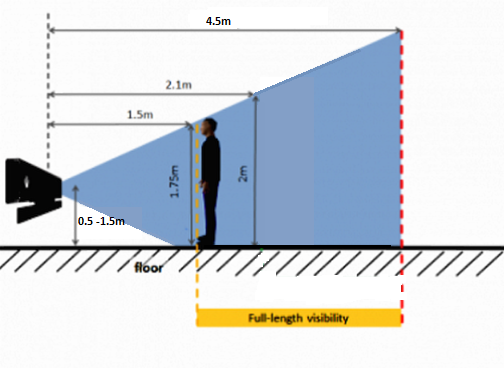
\includegraphics[scale=0.75]{exp.png}
\caption{Experimental Setup}

\end{figure}

\noindent The figure above gives us a nice visual representation of the setup\\
2) Firstly, the person is made to stand in a straight posture at the maximum range of Kinect (close to 4.5m). Here the static features readings are taken for a period of about 3 seconds\\
3) Then the person is asked to walk straight towards the Kinect. We are interested in the kinematic features of the walk upto a distance of 1.5m from the Kinect, because within this range we are able to capture the motion of the entire body. Beyond this,some part of the joints always goes out of the frame.\\
4) Although the range of 3m (4.5-1.5 m) appears small. It is more than adequate to extract one complete gait cycle. The representation of this gait cycle is shown in fig 5.1.\\




























